% Options for packages loaded elsewhere
% Options for packages loaded elsewhere
\PassOptionsToPackage{unicode}{hyperref}
\PassOptionsToPackage{hyphens}{url}
\PassOptionsToPackage{dvipsnames,svgnames,x11names}{xcolor}
%
\documentclass[
  letterpaper,
  DIV=11,
  numbers=noendperiod]{scrreprt}
\usepackage{xcolor}
\usepackage{amsmath,amssymb}
\setcounter{secnumdepth}{-\maxdimen} % remove section numbering
\usepackage{iftex}
\ifPDFTeX
  \usepackage[T1]{fontenc}
  \usepackage[utf8]{inputenc}
  \usepackage{textcomp} % provide euro and other symbols
\else % if luatex or xetex
  \usepackage{unicode-math} % this also loads fontspec
  \defaultfontfeatures{Scale=MatchLowercase}
  \defaultfontfeatures[\rmfamily]{Ligatures=TeX,Scale=1}
\fi
\usepackage{lmodern}
\ifPDFTeX\else
  % xetex/luatex font selection
\fi
% Use upquote if available, for straight quotes in verbatim environments
\IfFileExists{upquote.sty}{\usepackage{upquote}}{}
\IfFileExists{microtype.sty}{% use microtype if available
  \usepackage[]{microtype}
  \UseMicrotypeSet[protrusion]{basicmath} % disable protrusion for tt fonts
}{}
\makeatletter
\@ifundefined{KOMAClassName}{% if non-KOMA class
  \IfFileExists{parskip.sty}{%
    \usepackage{parskip}
  }{% else
    \setlength{\parindent}{0pt}
    \setlength{\parskip}{6pt plus 2pt minus 1pt}}
}{% if KOMA class
  \KOMAoptions{parskip=half}}
\makeatother
% Make \paragraph and \subparagraph free-standing
\makeatletter
\ifx\paragraph\undefined\else
  \let\oldparagraph\paragraph
  \renewcommand{\paragraph}{
    \@ifstar
      \xxxParagraphStar
      \xxxParagraphNoStar
  }
  \newcommand{\xxxParagraphStar}[1]{\oldparagraph*{#1}\mbox{}}
  \newcommand{\xxxParagraphNoStar}[1]{\oldparagraph{#1}\mbox{}}
\fi
\ifx\subparagraph\undefined\else
  \let\oldsubparagraph\subparagraph
  \renewcommand{\subparagraph}{
    \@ifstar
      \xxxSubParagraphStar
      \xxxSubParagraphNoStar
  }
  \newcommand{\xxxSubParagraphStar}[1]{\oldsubparagraph*{#1}\mbox{}}
  \newcommand{\xxxSubParagraphNoStar}[1]{\oldsubparagraph{#1}\mbox{}}
\fi
\makeatother


\usepackage{longtable,booktabs,array}
\newcounter{none} % for unnumbered tables
\usepackage{calc} % for calculating minipage widths
% Correct order of tables after \paragraph or \subparagraph
\usepackage{etoolbox}
\makeatletter
\patchcmd\longtable{\par}{\if@noskipsec\mbox{}\fi\par}{}{}
\makeatother
% Allow footnotes in longtable head/foot
\IfFileExists{footnotehyper.sty}{\usepackage{footnotehyper}}{\usepackage{footnote}}
\makesavenoteenv{longtable}
\usepackage{graphicx}
\makeatletter
\newsavebox\pandoc@box
\newcommand*\pandocbounded[1]{% scales image to fit in text height/width
  \sbox\pandoc@box{#1}%
  \Gscale@div\@tempa{\textheight}{\dimexpr\ht\pandoc@box+\dp\pandoc@box\relax}%
  \Gscale@div\@tempb{\linewidth}{\wd\pandoc@box}%
  \ifdim\@tempb\p@<\@tempa\p@\let\@tempa\@tempb\fi% select the smaller of both
  \ifdim\@tempa\p@<\p@\scalebox{\@tempa}{\usebox\pandoc@box}%
  \else\usebox{\pandoc@box}%
  \fi%
}
% Set default figure placement to htbp
\def\fps@figure{htbp}
\makeatother





\setlength{\emergencystretch}{3em} % prevent overfull lines

\providecommand{\tightlist}{%
  \setlength{\itemsep}{0pt}\setlength{\parskip}{0pt}}



 


\KOMAoption{captions}{tableheading}
\makeatletter
\@ifpackageloaded{tcolorbox}{}{\usepackage[skins,breakable]{tcolorbox}}
\@ifpackageloaded{fontawesome5}{}{\usepackage{fontawesome5}}
\definecolor{quarto-callout-color}{HTML}{909090}
\definecolor{quarto-callout-note-color}{HTML}{0758E5}
\definecolor{quarto-callout-important-color}{HTML}{CC1914}
\definecolor{quarto-callout-warning-color}{HTML}{EB9113}
\definecolor{quarto-callout-tip-color}{HTML}{00A047}
\definecolor{quarto-callout-caution-color}{HTML}{FC5300}
\definecolor{quarto-callout-color-frame}{HTML}{acacac}
\definecolor{quarto-callout-note-color-frame}{HTML}{4582ec}
\definecolor{quarto-callout-important-color-frame}{HTML}{d9534f}
\definecolor{quarto-callout-warning-color-frame}{HTML}{f0ad4e}
\definecolor{quarto-callout-tip-color-frame}{HTML}{02b875}
\definecolor{quarto-callout-caution-color-frame}{HTML}{fd7e14}
\makeatother
\makeatletter
\@ifpackageloaded{bookmark}{}{\usepackage{bookmark}}
\makeatother
\makeatletter
\@ifpackageloaded{caption}{}{\usepackage{caption}}
\AtBeginDocument{%
\ifdefined\contentsname
  \renewcommand*\contentsname{Table of contents}
\else
  \newcommand\contentsname{Table of contents}
\fi
\ifdefined\listfigurename
  \renewcommand*\listfigurename{List of Figures}
\else
  \newcommand\listfigurename{List of Figures}
\fi
\ifdefined\listtablename
  \renewcommand*\listtablename{List of Tables}
\else
  \newcommand\listtablename{List of Tables}
\fi
\ifdefined\figurename
  \renewcommand*\figurename{Figure}
\else
  \newcommand\figurename{Figure}
\fi
\ifdefined\tablename
  \renewcommand*\tablename{Table}
\else
  \newcommand\tablename{Table}
\fi
}
\@ifpackageloaded{float}{}{\usepackage{float}}
\floatstyle{ruled}
\@ifundefined{c@chapter}{\newfloat{codelisting}{h}{lop}}{\newfloat{codelisting}{h}{lop}[chapter]}
\floatname{codelisting}{Listing}
\newcommand*\listoflistings{\listof{codelisting}{List of Listings}}
\makeatother
\makeatletter
\makeatother
\makeatletter
\@ifpackageloaded{caption}{}{\usepackage{caption}}
\@ifpackageloaded{subcaption}{}{\usepackage{subcaption}}
\makeatother
\usepackage{bookmark}
\IfFileExists{xurl.sty}{\usepackage{xurl}}{} % add URL line breaks if available
\urlstyle{same}
\hypersetup{
  pdftitle={Jamovi Handbook},
  pdfauthor={{[}Your Name{]}},
  colorlinks=true,
  linkcolor={blue},
  filecolor={Maroon},
  citecolor={Blue},
  urlcolor={Blue},
  pdfcreator={LaTeX via pandoc}}


\title{Jamovi Handbook}
\usepackage{etoolbox}
\makeatletter
\providecommand{\subtitle}[1]{% add subtitle to \maketitle
  \apptocmd{\@title}{\par {\large #1 \par}}{}{}
}
\makeatother
\subtitle{A homework guide for {[}COURSE NUMBER{]}}
\author{{[}Your Name{]}}
\date{Invalid Date}
\begin{document}
\maketitle

\renewcommand*\contentsname{Table of contents}
{
\setcounter{tocdepth}{2}
\tableofcontents
}

\bookmarksetup{startatroot}

\chapter*{Welcome}\label{welcome}
\addcontentsline{toc}{chapter}{Welcome}

\markboth{Welcome}{Welcome}

This handbook is a homework guide for using \textbf{jamovi} in this
course. It is organized by task, not by menu. Start with the page that
matches the analysis named in your homework.

\begin{tcolorbox}[enhanced jigsaw, arc=.35mm, bottomrule=.15mm, breakable, colback=white, colframe=quarto-callout-important-color-frame, left=2mm, leftrule=.75mm, opacityback=0, rightrule=.15mm, toprule=.15mm]
\begin{minipage}[t]{5.5mm}
\textcolor{quarto-callout-important-color}{\faExclamation}
\end{minipage}%
\begin{minipage}[t]{\textwidth - 5.5mm}

\vspace{-3mm}\textbf{Use the course instructions first}\vspace{3mm}

This handbook explains how to run analyses in jamovi. Your homework
prompt tells you \textbf{which analysis to use}, \textbf{which variables
to analyze}, and \textbf{what to submit}.

\end{minipage}%
\end{tcolorbox}

\section*{How to use this handbook}\label{how-to-use-this-handbook}
\addcontentsline{toc}{section}{How to use this handbook}

\markright{How to use this handbook}

Each analysis page follows the same structure:

\begin{enumerate}
\def\labelenumi{\arabic{enumi}.}
\tightlist
\item
  \textbf{When to use it}
\item
  \textbf{Data requirements}
\item
  \textbf{Steps in jamovi}
\item
  \textbf{What to look at in the output}
\item
  \textbf{How to report the result}
\item
  \textbf{Common mistakes}
\end{enumerate}

\section*{What students usually need from each
output}\label{what-students-usually-need-from-each-output}
\addcontentsline{toc}{section}{What students usually need from each
output}

\markright{What students usually need from each output}

For most homework assignments, you will need some combination of:

{\def\LTcaptype{none} % do not increment counter
\begin{longtable}[]{@{}
  >{\raggedright\arraybackslash}p{(\linewidth - 2\tabcolsep) * \real{0.5000}}
  >{\raggedright\arraybackslash}p{(\linewidth - 2\tabcolsep) * \real{0.5000}}@{}}
\toprule\noalign{}
\begin{minipage}[b]{\linewidth}\raggedright
Output item
\end{minipage} & \begin{minipage}[b]{\linewidth}\raggedright
Why it matters
\end{minipage} \\
\midrule\noalign{}
\endhead
\bottomrule\noalign{}
\endlastfoot
Test statistic & The main statistic, such as \emph{t}, \emph{F},
\emph{r}, or \emph{b} \\
Degrees of freedom & Needed for many APA-style writeups \\
\emph{p}-value & Used to evaluate statistical significance \\
Effect size & Describes the size of the effect \\
Confidence interval & Gives a range of plausible values \\
Descriptive statistics & Helps interpret the direction and size of the
result \\
\end{longtable}
}

\section*{Suggested workflow}\label{suggested-workflow}
\addcontentsline{toc}{section}{Suggested workflow}

\markright{Suggested workflow}

\begin{enumerate}
\def\labelenumi{\arabic{enumi}.}
\tightlist
\item
  Open the data file.
\item
  Check the variable types and labels.
\item
  Run the analysis.
\item
  Check assumptions, if required.
\item
  Identify the relevant output table.
\item
  Write the result in plain language.
\item
  Use the course reporting template.
\end{enumerate}

\part{Start Here}

\chapter{Installing or Opening
jamovi}\label{installing-or-opening-jamovi}

\begin{tcolorbox}[enhanced jigsaw, arc=.35mm, bottomrule=.15mm, breakable, colback=white, colframe=quarto-callout-note-color-frame, left=2mm, leftrule=.75mm, opacityback=0, rightrule=.15mm, toprule=.15mm]
\begin{minipage}[t]{5.5mm}
\textcolor{quarto-callout-note-color}{\faInfo}
\end{minipage}%
\begin{minipage}[t]{\textwidth - 5.5mm}

\vspace{-3mm}\textbf{Draft page}\vspace{3mm}

Use this page as a placeholder. Replace this note with the
procedure-specific instructions students need for your homework.

\end{minipage}%
\end{tcolorbox}

\section{When to use this}\label{when-to-use-this}

Describe the type of research question this analysis answers.

\section{Data requirements}\label{data-requirements}

{\def\LTcaptype{none} % do not increment counter
\begin{longtable}[]{@{}
  >{\raggedright\arraybackslash}p{(\linewidth - 2\tabcolsep) * \real{0.5000}}
  >{\raggedright\arraybackslash}p{(\linewidth - 2\tabcolsep) * \real{0.5000}}@{}}
\toprule\noalign{}
\begin{minipage}[b]{\linewidth}\raggedright
Requirement
\end{minipage} & \begin{minipage}[b]{\linewidth}\raggedright
What students should check
\end{minipage} \\
\midrule\noalign{}
\endhead
\bottomrule\noalign{}
\endlastfoot
Outcome variable & Replace with required variable type \\
Predictor/grouping variable & Replace with required variable type \\
Observations & Replace with independence/repeated-measures
requirement \\
Missing values & State course rule \\
\end{longtable}
}

\section{Steps in jamovi}\label{steps-in-jamovi}

\begin{enumerate}
\def\labelenumi{\arabic{enumi}.}
\tightlist
\item
  Open the homework data file.
\item
  Select the correct analysis menu.
\item
  Move the required variables into the correct boxes.
\item
  Select the options required by the homework.
\item
  Check the output table named in the homework.
\end{enumerate}

\section{What to report}\label{what-to-report}

\begin{itemize}
\tightlist
\item
  Test statistic:
\item
  Degrees of freedom:
\item
  \emph{p}-value:
\item
  Effect size:
\item
  Confidence interval, if required:
\end{itemize}

\section{Common mistakes}\label{common-mistakes}

\begin{tcolorbox}[enhanced jigsaw, arc=.35mm, bottomrule=.15mm, breakable, colback=white, colframe=quarto-callout-warning-color-frame, left=2mm, leftrule=.75mm, opacityback=0, rightrule=.15mm, toprule=.15mm]
\begin{minipage}[t]{5.5mm}
\textcolor{quarto-callout-warning-color}{\faExclamationTriangle}
\end{minipage}%
\begin{minipage}[t]{\textwidth - 5.5mm}

\vspace{-3mm}\textbf{Watch for this}\vspace{3mm}

List one or two mistakes students commonly make on this assignment.

\end{minipage}%
\end{tcolorbox}

\chapter{Opening Data Files}\label{opening-data-files}

\begin{tcolorbox}[enhanced jigsaw, arc=.35mm, bottomrule=.15mm, breakable, colback=white, colframe=quarto-callout-note-color-frame, left=2mm, leftrule=.75mm, opacityback=0, rightrule=.15mm, toprule=.15mm]
\begin{minipage}[t]{5.5mm}
\textcolor{quarto-callout-note-color}{\faInfo}
\end{minipage}%
\begin{minipage}[t]{\textwidth - 5.5mm}

\vspace{-3mm}\textbf{Draft page}\vspace{3mm}

Use this page as a placeholder. Replace this note with the
procedure-specific instructions students need for your homework.

\end{minipage}%
\end{tcolorbox}

\section{When to use this}\label{when-to-use-this-1}

Describe the type of research question this analysis answers.

\section{Data requirements}\label{data-requirements-1}

{\def\LTcaptype{none} % do not increment counter
\begin{longtable}[]{@{}
  >{\raggedright\arraybackslash}p{(\linewidth - 2\tabcolsep) * \real{0.5000}}
  >{\raggedright\arraybackslash}p{(\linewidth - 2\tabcolsep) * \real{0.5000}}@{}}
\toprule\noalign{}
\begin{minipage}[b]{\linewidth}\raggedright
Requirement
\end{minipage} & \begin{minipage}[b]{\linewidth}\raggedright
What students should check
\end{minipage} \\
\midrule\noalign{}
\endhead
\bottomrule\noalign{}
\endlastfoot
Outcome variable & Replace with required variable type \\
Predictor/grouping variable & Replace with required variable type \\
Observations & Replace with independence/repeated-measures
requirement \\
Missing values & State course rule \\
\end{longtable}
}

\section{Steps in jamovi}\label{steps-in-jamovi-1}

\begin{enumerate}
\def\labelenumi{\arabic{enumi}.}
\tightlist
\item
  Open the homework data file.
\item
  Select the correct analysis menu.
\item
  Move the required variables into the correct boxes.
\item
  Select the options required by the homework.
\item
  Check the output table named in the homework.
\end{enumerate}

\section{What to report}\label{what-to-report-1}

\begin{itemize}
\tightlist
\item
  Test statistic:
\item
  Degrees of freedom:
\item
  \emph{p}-value:
\item
  Effect size:
\item
  Confidence interval, if required:
\end{itemize}

\section{Common mistakes}\label{common-mistakes-1}

\begin{tcolorbox}[enhanced jigsaw, arc=.35mm, bottomrule=.15mm, breakable, colback=white, colframe=quarto-callout-warning-color-frame, left=2mm, leftrule=.75mm, opacityback=0, rightrule=.15mm, toprule=.15mm]
\begin{minipage}[t]{5.5mm}
\textcolor{quarto-callout-warning-color}{\faExclamationTriangle}
\end{minipage}%
\begin{minipage}[t]{\textwidth - 5.5mm}

\vspace{-3mm}\textbf{Watch for this}\vspace{3mm}

List one or two mistakes students commonly make on this assignment.

\end{minipage}%
\end{tcolorbox}

\chapter{Checking Variable Types}\label{checking-variable-types}

\begin{tcolorbox}[enhanced jigsaw, arc=.35mm, bottomrule=.15mm, breakable, colback=white, colframe=quarto-callout-note-color-frame, left=2mm, leftrule=.75mm, opacityback=0, rightrule=.15mm, toprule=.15mm]
\begin{minipage}[t]{5.5mm}
\textcolor{quarto-callout-note-color}{\faInfo}
\end{minipage}%
\begin{minipage}[t]{\textwidth - 5.5mm}

\vspace{-3mm}\textbf{Draft page}\vspace{3mm}

Use this page as a placeholder. Replace this note with the
procedure-specific instructions students need for your homework.

\end{minipage}%
\end{tcolorbox}

\section{When to use this}\label{when-to-use-this-2}

Describe the type of research question this analysis answers.

\section{Data requirements}\label{data-requirements-2}

{\def\LTcaptype{none} % do not increment counter
\begin{longtable}[]{@{}
  >{\raggedright\arraybackslash}p{(\linewidth - 2\tabcolsep) * \real{0.5000}}
  >{\raggedright\arraybackslash}p{(\linewidth - 2\tabcolsep) * \real{0.5000}}@{}}
\toprule\noalign{}
\begin{minipage}[b]{\linewidth}\raggedright
Requirement
\end{minipage} & \begin{minipage}[b]{\linewidth}\raggedright
What students should check
\end{minipage} \\
\midrule\noalign{}
\endhead
\bottomrule\noalign{}
\endlastfoot
Outcome variable & Replace with required variable type \\
Predictor/grouping variable & Replace with required variable type \\
Observations & Replace with independence/repeated-measures
requirement \\
Missing values & State course rule \\
\end{longtable}
}

\section{Steps in jamovi}\label{steps-in-jamovi-2}

\begin{enumerate}
\def\labelenumi{\arabic{enumi}.}
\tightlist
\item
  Open the homework data file.
\item
  Select the correct analysis menu.
\item
  Move the required variables into the correct boxes.
\item
  Select the options required by the homework.
\item
  Check the output table named in the homework.
\end{enumerate}

\section{What to report}\label{what-to-report-2}

\begin{itemize}
\tightlist
\item
  Test statistic:
\item
  Degrees of freedom:
\item
  \emph{p}-value:
\item
  Effect size:
\item
  Confidence interval, if required:
\end{itemize}

\section{Common mistakes}\label{common-mistakes-2}

\begin{tcolorbox}[enhanced jigsaw, arc=.35mm, bottomrule=.15mm, breakable, colback=white, colframe=quarto-callout-warning-color-frame, left=2mm, leftrule=.75mm, opacityback=0, rightrule=.15mm, toprule=.15mm]
\begin{minipage}[t]{5.5mm}
\textcolor{quarto-callout-warning-color}{\faExclamationTriangle}
\end{minipage}%
\begin{minipage}[t]{\textwidth - 5.5mm}

\vspace{-3mm}\textbf{Watch for this}\vspace{3mm}

List one or two mistakes students commonly make on this assignment.

\end{minipage}%
\end{tcolorbox}

\part{Describing Data}

\chapter{Descriptive Statistics}\label{descriptive-statistics}

\begin{tcolorbox}[enhanced jigsaw, arc=.35mm, bottomrule=.15mm, breakable, colback=white, colframe=quarto-callout-note-color-frame, left=2mm, leftrule=.75mm, opacityback=0, rightrule=.15mm, toprule=.15mm]
\begin{minipage}[t]{5.5mm}
\textcolor{quarto-callout-note-color}{\faInfo}
\end{minipage}%
\begin{minipage}[t]{\textwidth - 5.5mm}

\vspace{-3mm}\textbf{Draft page}\vspace{3mm}

Use this page as a placeholder. Replace this note with the
procedure-specific instructions students need for your homework.

\end{minipage}%
\end{tcolorbox}

\section{When to use this}\label{when-to-use-this-3}

Describe the type of research question this analysis answers.

\section{Data requirements}\label{data-requirements-3}

{\def\LTcaptype{none} % do not increment counter
\begin{longtable}[]{@{}
  >{\raggedright\arraybackslash}p{(\linewidth - 2\tabcolsep) * \real{0.5000}}
  >{\raggedright\arraybackslash}p{(\linewidth - 2\tabcolsep) * \real{0.5000}}@{}}
\toprule\noalign{}
\begin{minipage}[b]{\linewidth}\raggedright
Requirement
\end{minipage} & \begin{minipage}[b]{\linewidth}\raggedright
What students should check
\end{minipage} \\
\midrule\noalign{}
\endhead
\bottomrule\noalign{}
\endlastfoot
Outcome variable & Replace with required variable type \\
Predictor/grouping variable & Replace with required variable type \\
Observations & Replace with independence/repeated-measures
requirement \\
Missing values & State course rule \\
\end{longtable}
}

\section{Steps in jamovi}\label{steps-in-jamovi-3}

\begin{enumerate}
\def\labelenumi{\arabic{enumi}.}
\tightlist
\item
  Open the homework data file.
\item
  Select the correct analysis menu.
\item
  Move the required variables into the correct boxes.
\item
  Select the options required by the homework.
\item
  Check the output table named in the homework.
\end{enumerate}

\section{What to report}\label{what-to-report-3}

\begin{itemize}
\tightlist
\item
  Test statistic:
\item
  Degrees of freedom:
\item
  \emph{p}-value:
\item
  Effect size:
\item
  Confidence interval, if required:
\end{itemize}

\section{Common mistakes}\label{common-mistakes-3}

\begin{tcolorbox}[enhanced jigsaw, arc=.35mm, bottomrule=.15mm, breakable, colback=white, colframe=quarto-callout-warning-color-frame, left=2mm, leftrule=.75mm, opacityback=0, rightrule=.15mm, toprule=.15mm]
\begin{minipage}[t]{5.5mm}
\textcolor{quarto-callout-warning-color}{\faExclamationTriangle}
\end{minipage}%
\begin{minipage}[t]{\textwidth - 5.5mm}

\vspace{-3mm}\textbf{Watch for this}\vspace{3mm}

List one or two mistakes students commonly make on this assignment.

\end{minipage}%
\end{tcolorbox}

\chapter{Graphs and Plots}\label{graphs-and-plots}

\begin{tcolorbox}[enhanced jigsaw, arc=.35mm, bottomrule=.15mm, breakable, colback=white, colframe=quarto-callout-note-color-frame, left=2mm, leftrule=.75mm, opacityback=0, rightrule=.15mm, toprule=.15mm]
\begin{minipage}[t]{5.5mm}
\textcolor{quarto-callout-note-color}{\faInfo}
\end{minipage}%
\begin{minipage}[t]{\textwidth - 5.5mm}

\vspace{-3mm}\textbf{Draft page}\vspace{3mm}

Use this page as a placeholder. Replace this note with the
procedure-specific instructions students need for your homework.

\end{minipage}%
\end{tcolorbox}

\section{When to use this}\label{when-to-use-this-4}

Describe the type of research question this analysis answers.

\section{Data requirements}\label{data-requirements-4}

{\def\LTcaptype{none} % do not increment counter
\begin{longtable}[]{@{}
  >{\raggedright\arraybackslash}p{(\linewidth - 2\tabcolsep) * \real{0.5000}}
  >{\raggedright\arraybackslash}p{(\linewidth - 2\tabcolsep) * \real{0.5000}}@{}}
\toprule\noalign{}
\begin{minipage}[b]{\linewidth}\raggedright
Requirement
\end{minipage} & \begin{minipage}[b]{\linewidth}\raggedright
What students should check
\end{minipage} \\
\midrule\noalign{}
\endhead
\bottomrule\noalign{}
\endlastfoot
Outcome variable & Replace with required variable type \\
Predictor/grouping variable & Replace with required variable type \\
Observations & Replace with independence/repeated-measures
requirement \\
Missing values & State course rule \\
\end{longtable}
}

\section{Steps in jamovi}\label{steps-in-jamovi-4}

\begin{enumerate}
\def\labelenumi{\arabic{enumi}.}
\tightlist
\item
  Open the homework data file.
\item
  Select the correct analysis menu.
\item
  Move the required variables into the correct boxes.
\item
  Select the options required by the homework.
\item
  Check the output table named in the homework.
\end{enumerate}

\section{What to report}\label{what-to-report-4}

\begin{itemize}
\tightlist
\item
  Test statistic:
\item
  Degrees of freedom:
\item
  \emph{p}-value:
\item
  Effect size:
\item
  Confidence interval, if required:
\end{itemize}

\section{Common mistakes}\label{common-mistakes-4}

\begin{tcolorbox}[enhanced jigsaw, arc=.35mm, bottomrule=.15mm, breakable, colback=white, colframe=quarto-callout-warning-color-frame, left=2mm, leftrule=.75mm, opacityback=0, rightrule=.15mm, toprule=.15mm]
\begin{minipage}[t]{5.5mm}
\textcolor{quarto-callout-warning-color}{\faExclamationTriangle}
\end{minipage}%
\begin{minipage}[t]{\textwidth - 5.5mm}

\vspace{-3mm}\textbf{Watch for this}\vspace{3mm}

List one or two mistakes students commonly make on this assignment.

\end{minipage}%
\end{tcolorbox}

\part{Group Comparisons}

\chapter{Independent-Samples t-Test}\label{independent-samples-t-test}

Use this page when a homework problem asks whether \textbf{two
independent groups} differ on a \textbf{continuous outcome variable}.

\begin{tcolorbox}[enhanced jigsaw, arc=.35mm, bottomrule=.15mm, breakable, colback=white, colframe=quarto-callout-tip-color-frame, left=2mm, leftrule=.75mm, opacityback=0, rightrule=.15mm, toprule=.15mm]
\begin{minipage}[t]{5.5mm}
\textcolor{quarto-callout-tip-color}{\faLightbulb}
\end{minipage}%
\begin{minipage}[t]{\textwidth - 5.5mm}

\vspace{-3mm}\textbf{Fast decision rule}\vspace{3mm}

Use an independent-samples t-test when you have:

\begin{itemize}
\tightlist
\item
  one quantitative outcome, such as test score, anxiety score, reaction
  time, or income
\item
  one grouping variable with two independent groups, such as
  treatment/control or online/in-person
\end{itemize}

\end{minipage}%
\end{tcolorbox}

\section{Example research question}\label{example-research-question}

Do students in the online section and face-to-face section differ in
final exam scores?

\section{Data requirements}\label{data-requirements-5}

{\def\LTcaptype{none} % do not increment counter
\begin{longtable}[]{@{}
  >{\raggedright\arraybackslash}p{(\linewidth - 4\tabcolsep) * \real{0.3333}}
  >{\raggedright\arraybackslash}p{(\linewidth - 4\tabcolsep) * \real{0.3333}}
  >{\raggedright\arraybackslash}p{(\linewidth - 4\tabcolsep) * \real{0.3333}}@{}}
\toprule\noalign{}
\begin{minipage}[b]{\linewidth}\raggedright
Item
\end{minipage} & \begin{minipage}[b]{\linewidth}\raggedright
Requirement
\end{minipage} & \begin{minipage}[b]{\linewidth}\raggedright
Example
\end{minipage} \\
\midrule\noalign{}
\endhead
\bottomrule\noalign{}
\endlastfoot
Outcome variable & Continuous / scale variable &
\texttt{final\_exam\_score} \\
Grouping variable & Two independent groups & \texttt{section\_type}:
online vs.~face-to-face \\
Observations & Each person appears in only one group & A student is not
in both sections \\
Main question & Compare the two group means & Is one group's mean
higher? \\
\end{longtable}
}

\begin{tcolorbox}[enhanced jigsaw, arc=.35mm, bottomrule=.15mm, breakable, colback=white, colframe=quarto-callout-warning-color-frame, left=2mm, leftrule=.75mm, opacityback=0, rightrule=.15mm, toprule=.15mm]
\begin{minipage}[t]{5.5mm}
\textcolor{quarto-callout-warning-color}{\faExclamationTriangle}
\end{minipage}%
\begin{minipage}[t]{\textwidth - 5.5mm}

\vspace{-3mm}\textbf{Do not use this test when}\vspace{3mm}

Do not use this test when the same people are measured twice. For
before/after scores from the same students, use a \textbf{paired-samples
t-test} instead.

\end{minipage}%
\end{tcolorbox}

\section{Steps in jamovi}\label{steps-in-jamovi-5}

{\def\LTcaptype{none} % do not increment counter
\begin{longtable}[]{@{}
  >{\raggedleft\arraybackslash}p{(\linewidth - 2\tabcolsep) * \real{0.5714}}
  >{\raggedright\arraybackslash}p{(\linewidth - 2\tabcolsep) * \real{0.4286}}@{}}
\toprule\noalign{}
\begin{minipage}[b]{\linewidth}\raggedleft
Step
\end{minipage} & \begin{minipage}[b]{\linewidth}\raggedright
What to do
\end{minipage} \\
\midrule\noalign{}
\endhead
\bottomrule\noalign{}
\endlastfoot
1 & Open the homework data file in jamovi. \\
2 & Go to \textbf{Analyses \textgreater{} T-Tests \textgreater{}
Independent Samples T-Test}. \\
3 & Move the continuous outcome variable into \textbf{Dependent
Variables}. \\
4 & Move the two-group variable into \textbf{Grouping Variable}. \\
5 & Select the options required by the homework, such as descriptives,
confidence interval, effect size, or assumption checks. \\
6 & Read the output table named \textbf{Independent Samples T-Test}. \\
\end{longtable}
}

\section{Screenshot: setup}\label{screenshot-setup}

Replace Figure~\ref{fig-independent-ttest-setup} with your own jamovi
screenshot once you capture it.

\begin{figure}

\centering{

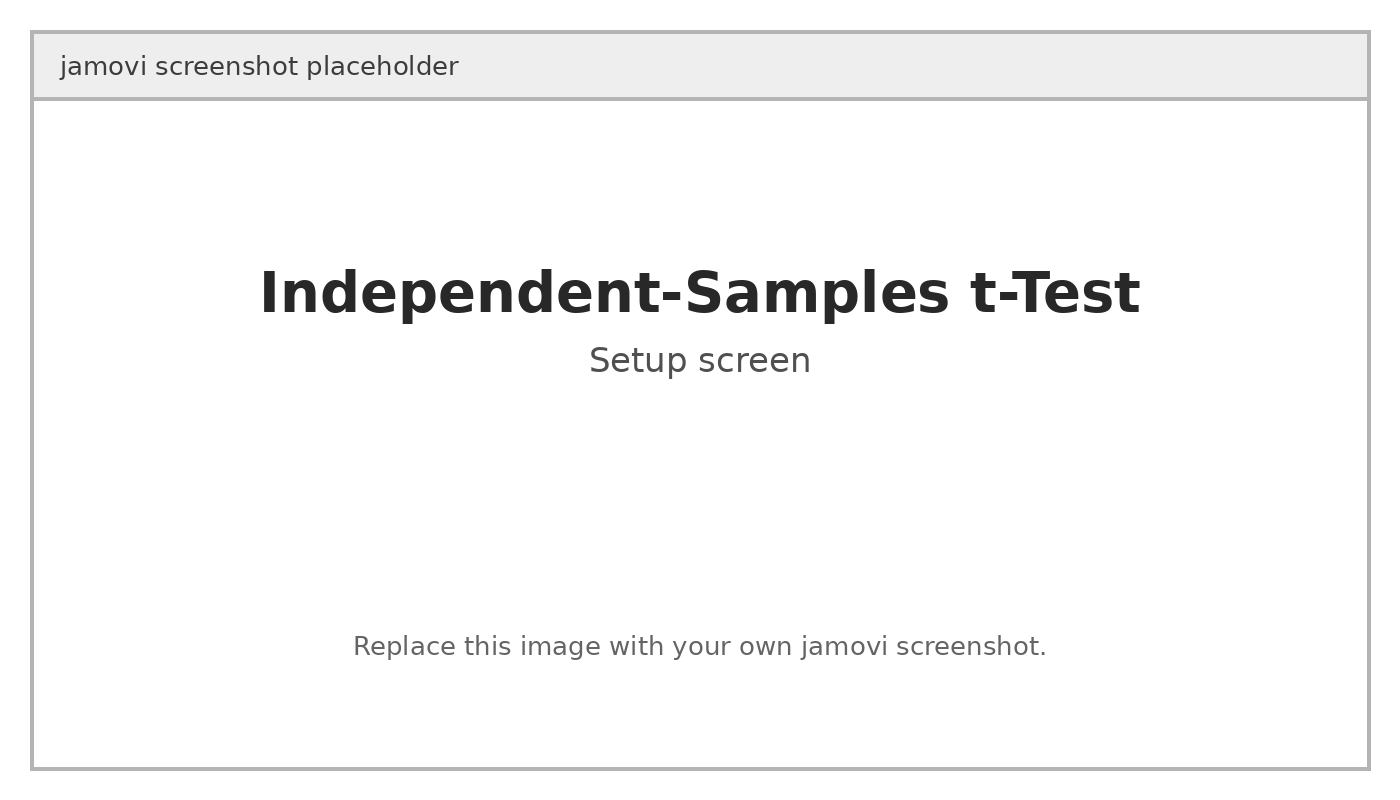
\includegraphics[width=0.9\linewidth,height=\textheight,keepaspectratio,alt={Placeholder image for the jamovi independent-samples t-test setup screen.}]{images/20-independent-ttest-dialog.png}

}

\caption{\label{fig-independent-ttest-setup}Placeholder for the jamovi
independent-samples t-test setup screen.}

\end{figure}%

\section{What to look at in the
output}\label{what-to-look-at-in-the-output}

\begin{figure}

\centering{

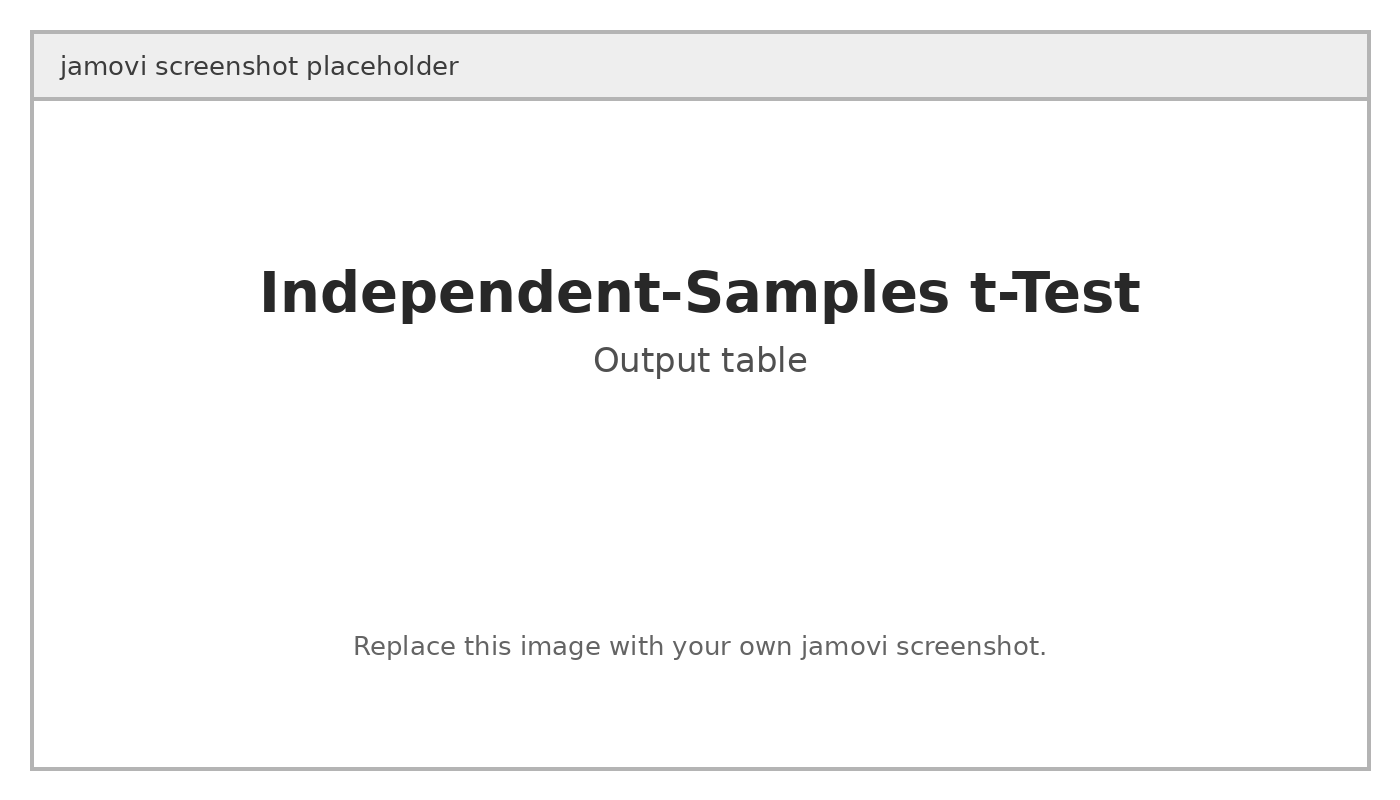
\includegraphics[width=0.9\linewidth,height=\textheight,keepaspectratio,alt={Placeholder image for the jamovi independent-samples t-test output table.}]{images/20-independent-ttest-output.png}

}

\caption{\label{fig-independent-ttest-output}Placeholder for the jamovi
independent-samples t-test output table.}

\end{figure}%

Use the output table to find:

{\def\LTcaptype{none} % do not increment counter
\begin{longtable}[]{@{}ll@{}}
\toprule\noalign{}
Output item & Where students should look \\
\midrule\noalign{}
\endhead
\bottomrule\noalign{}
\endlastfoot
Test statistic & The column labeled something like \texttt{statistic} \\
Degrees of freedom & The \texttt{df} column \\
\emph{p}-value & The \texttt{p} column \\
Group means & The descriptives table, if selected \\
Confidence interval & The confidence interval columns, if selected \\
Effect size & The effect size column, if selected \\
\end{longtable}
}

\section{How to decide what the result
means}\label{how-to-decide-what-the-result-means}

\begin{tcolorbox}[enhanced jigsaw, arc=.35mm, bottomrule=.15mm, breakable, colback=white, colframe=quarto-callout-note-color-frame, left=2mm, leftrule=.75mm, opacityback=0, rightrule=.15mm, toprule=.15mm]
\begin{minipage}[t]{5.5mm}
\textcolor{quarto-callout-note-color}{\faInfo}
\end{minipage}%
\begin{minipage}[t]{\textwidth - 5.5mm}

\vspace{-3mm}\textbf{Course rule}\vspace{3mm}

Use the significance level assigned by your instructor. In many
introductory courses, this is \(\alpha = .05\).

\end{minipage}%
\end{tcolorbox}

A typical interpretation has three parts:

\begin{enumerate}
\def\labelenumi{\arabic{enumi}.}
\tightlist
\item
  State whether the result is statistically significant.
\item
  State which group had the higher/lower mean.
\item
  State what that means in the context of the research question.
\end{enumerate}

\section{Reporting template}\label{reporting-template}

Use this template, replacing the bracketed text with your result:

\begin{quote}
An independent-samples t-test was conducted to compare
\textbf{{[}outcome variable{]}} between \textbf{{[}Group 1{]}} and
\textbf{{[}Group 2{]}}. The difference between groups was
\textbf{{[}statistically significant / not statistically
significant{]}}, \emph{t}(\emph{df}) = \textbf{{[}t value{]}}, \emph{p}
= \textbf{{[}p value{]}}. Students in \textbf{{[}group with higher
mean{]}} had a \textbf{{[}higher/lower{]}} mean score (\emph{M} =
\textbf{{[}mean{]}}) than students in \textbf{{[}other group{]}}
(\emph{M} = \textbf{{[}mean{]}}).
\end{quote}

If your homework asks for effect size, add:

\begin{quote}
The effect size was \textbf{{[}small / medium / large, if your course
uses those labels{]}}, Cohen's \emph{d} = \textbf{{[}value{]}}.
\end{quote}

\section{Common mistakes}\label{common-mistakes-5}

\begin{tcolorbox}[enhanced jigsaw, arc=.35mm, bottomrule=.15mm, breakable, colback=white, colframe=quarto-callout-warning-color-frame, left=2mm, leftrule=.75mm, opacityback=0, rightrule=.15mm, toprule=.15mm]
\begin{minipage}[t]{5.5mm}
\textcolor{quarto-callout-warning-color}{\faExclamationTriangle}
\end{minipage}%
\begin{minipage}[t]{\textwidth - 5.5mm}

\vspace{-3mm}\textbf{Mistake 1: Reversing the variables}\vspace{3mm}

The outcome goes in \textbf{Dependent Variables}. The two-group variable
goes in \textbf{Grouping Variable}.

\end{minipage}%
\end{tcolorbox}

\begin{tcolorbox}[enhanced jigsaw, arc=.35mm, bottomrule=.15mm, breakable, colback=white, colframe=quarto-callout-warning-color-frame, left=2mm, leftrule=.75mm, opacityback=0, rightrule=.15mm, toprule=.15mm]
\begin{minipage}[t]{5.5mm}
\textcolor{quarto-callout-warning-color}{\faExclamationTriangle}
\end{minipage}%
\begin{minipage}[t]{\textwidth - 5.5mm}

\vspace{-3mm}\textbf{Mistake 2: Using a paired t-test instead}\vspace{3mm}

Use a paired-samples t-test only when the same cases are measured twice
or matched in pairs.

\end{minipage}%
\end{tcolorbox}

\begin{tcolorbox}[enhanced jigsaw, arc=.35mm, bottomrule=.15mm, breakable, colback=white, colframe=quarto-callout-warning-color-frame, left=2mm, leftrule=.75mm, opacityback=0, rightrule=.15mm, toprule=.15mm]
\begin{minipage}[t]{5.5mm}
\textcolor{quarto-callout-warning-color}{\faExclamationTriangle}
\end{minipage}%
\begin{minipage}[t]{\textwidth - 5.5mm}

\vspace{-3mm}\textbf{Mistake 3: Reporting only the p-value}\vspace{3mm}

A complete homework answer usually needs the test statistic, degrees of
freedom, p-value, and a plain-language interpretation.

\end{minipage}%
\end{tcolorbox}

\section{Student checklist}\label{student-checklist}

Before submitting, confirm that you have:

\begin{itemize}
\tightlist
\item[$\square$]
  Used the correct test
\item[$\square$]
  Put the variables in the correct boxes
\item[$\square$]
  Reported the relevant statistic
\item[$\square$]
  Reported the p-value
\item[$\square$]
  Interpreted the result in context
\item[$\square$]
  Included effect size or confidence interval if required
\end{itemize}

\chapter{Paired-Samples t-Test}\label{paired-samples-t-test}

\begin{tcolorbox}[enhanced jigsaw, arc=.35mm, bottomrule=.15mm, breakable, colback=white, colframe=quarto-callout-note-color-frame, left=2mm, leftrule=.75mm, opacityback=0, rightrule=.15mm, toprule=.15mm]
\begin{minipage}[t]{5.5mm}
\textcolor{quarto-callout-note-color}{\faInfo}
\end{minipage}%
\begin{minipage}[t]{\textwidth - 5.5mm}

\vspace{-3mm}\textbf{Draft page}\vspace{3mm}

Use this page as a placeholder. Replace this note with the
procedure-specific instructions students need for your homework.

\end{minipage}%
\end{tcolorbox}

\section{When to use this}\label{when-to-use-this-5}

Describe the type of research question this analysis answers.

\section{Data requirements}\label{data-requirements-6}

{\def\LTcaptype{none} % do not increment counter
\begin{longtable}[]{@{}
  >{\raggedright\arraybackslash}p{(\linewidth - 2\tabcolsep) * \real{0.5000}}
  >{\raggedright\arraybackslash}p{(\linewidth - 2\tabcolsep) * \real{0.5000}}@{}}
\toprule\noalign{}
\begin{minipage}[b]{\linewidth}\raggedright
Requirement
\end{minipage} & \begin{minipage}[b]{\linewidth}\raggedright
What students should check
\end{minipage} \\
\midrule\noalign{}
\endhead
\bottomrule\noalign{}
\endlastfoot
Outcome variable & Replace with required variable type \\
Predictor/grouping variable & Replace with required variable type \\
Observations & Replace with independence/repeated-measures
requirement \\
Missing values & State course rule \\
\end{longtable}
}

\section{Steps in jamovi}\label{steps-in-jamovi-6}

\begin{enumerate}
\def\labelenumi{\arabic{enumi}.}
\tightlist
\item
  Open the homework data file.
\item
  Select the correct analysis menu.
\item
  Move the required variables into the correct boxes.
\item
  Select the options required by the homework.
\item
  Check the output table named in the homework.
\end{enumerate}

\section{What to report}\label{what-to-report-5}

\begin{itemize}
\tightlist
\item
  Test statistic:
\item
  Degrees of freedom:
\item
  \emph{p}-value:
\item
  Effect size:
\item
  Confidence interval, if required:
\end{itemize}

\section{Common mistakes}\label{common-mistakes-6}

\begin{tcolorbox}[enhanced jigsaw, arc=.35mm, bottomrule=.15mm, breakable, colback=white, colframe=quarto-callout-warning-color-frame, left=2mm, leftrule=.75mm, opacityback=0, rightrule=.15mm, toprule=.15mm]
\begin{minipage}[t]{5.5mm}
\textcolor{quarto-callout-warning-color}{\faExclamationTriangle}
\end{minipage}%
\begin{minipage}[t]{\textwidth - 5.5mm}

\vspace{-3mm}\textbf{Watch for this}\vspace{3mm}

List one or two mistakes students commonly make on this assignment.

\end{minipage}%
\end{tcolorbox}

\chapter{One-Way ANOVA}\label{one-way-anova}

\begin{tcolorbox}[enhanced jigsaw, arc=.35mm, bottomrule=.15mm, breakable, colback=white, colframe=quarto-callout-note-color-frame, left=2mm, leftrule=.75mm, opacityback=0, rightrule=.15mm, toprule=.15mm]
\begin{minipage}[t]{5.5mm}
\textcolor{quarto-callout-note-color}{\faInfo}
\end{minipage}%
\begin{minipage}[t]{\textwidth - 5.5mm}

\vspace{-3mm}\textbf{Draft page}\vspace{3mm}

Use this page as a placeholder. Replace this note with the
procedure-specific instructions students need for your homework.

\end{minipage}%
\end{tcolorbox}

\section{When to use this}\label{when-to-use-this-6}

Describe the type of research question this analysis answers.

\section{Data requirements}\label{data-requirements-7}

{\def\LTcaptype{none} % do not increment counter
\begin{longtable}[]{@{}
  >{\raggedright\arraybackslash}p{(\linewidth - 2\tabcolsep) * \real{0.5000}}
  >{\raggedright\arraybackslash}p{(\linewidth - 2\tabcolsep) * \real{0.5000}}@{}}
\toprule\noalign{}
\begin{minipage}[b]{\linewidth}\raggedright
Requirement
\end{minipage} & \begin{minipage}[b]{\linewidth}\raggedright
What students should check
\end{minipage} \\
\midrule\noalign{}
\endhead
\bottomrule\noalign{}
\endlastfoot
Outcome variable & Replace with required variable type \\
Predictor/grouping variable & Replace with required variable type \\
Observations & Replace with independence/repeated-measures
requirement \\
Missing values & State course rule \\
\end{longtable}
}

\section{Steps in jamovi}\label{steps-in-jamovi-7}

\begin{enumerate}
\def\labelenumi{\arabic{enumi}.}
\tightlist
\item
  Open the homework data file.
\item
  Select the correct analysis menu.
\item
  Move the required variables into the correct boxes.
\item
  Select the options required by the homework.
\item
  Check the output table named in the homework.
\end{enumerate}

\section{What to report}\label{what-to-report-6}

\begin{itemize}
\tightlist
\item
  Test statistic:
\item
  Degrees of freedom:
\item
  \emph{p}-value:
\item
  Effect size:
\item
  Confidence interval, if required:
\end{itemize}

\section{Common mistakes}\label{common-mistakes-7}

\begin{tcolorbox}[enhanced jigsaw, arc=.35mm, bottomrule=.15mm, breakable, colback=white, colframe=quarto-callout-warning-color-frame, left=2mm, leftrule=.75mm, opacityback=0, rightrule=.15mm, toprule=.15mm]
\begin{minipage}[t]{5.5mm}
\textcolor{quarto-callout-warning-color}{\faExclamationTriangle}
\end{minipage}%
\begin{minipage}[t]{\textwidth - 5.5mm}

\vspace{-3mm}\textbf{Watch for this}\vspace{3mm}

List one or two mistakes students commonly make on this assignment.

\end{minipage}%
\end{tcolorbox}

\chapter{Multiple Comparisons}\label{multiple-comparisons}

\begin{tcolorbox}[enhanced jigsaw, arc=.35mm, bottomrule=.15mm, breakable, colback=white, colframe=quarto-callout-note-color-frame, left=2mm, leftrule=.75mm, opacityback=0, rightrule=.15mm, toprule=.15mm]
\begin{minipage}[t]{5.5mm}
\textcolor{quarto-callout-note-color}{\faInfo}
\end{minipage}%
\begin{minipage}[t]{\textwidth - 5.5mm}

\vspace{-3mm}\textbf{Draft page}\vspace{3mm}

Use this page as a placeholder. Replace this note with the
procedure-specific instructions students need for your homework.

\end{minipage}%
\end{tcolorbox}

\section{When to use this}\label{when-to-use-this-7}

Describe the type of research question this analysis answers.

\section{Data requirements}\label{data-requirements-8}

{\def\LTcaptype{none} % do not increment counter
\begin{longtable}[]{@{}
  >{\raggedright\arraybackslash}p{(\linewidth - 2\tabcolsep) * \real{0.5000}}
  >{\raggedright\arraybackslash}p{(\linewidth - 2\tabcolsep) * \real{0.5000}}@{}}
\toprule\noalign{}
\begin{minipage}[b]{\linewidth}\raggedright
Requirement
\end{minipage} & \begin{minipage}[b]{\linewidth}\raggedright
What students should check
\end{minipage} \\
\midrule\noalign{}
\endhead
\bottomrule\noalign{}
\endlastfoot
Outcome variable & Replace with required variable type \\
Predictor/grouping variable & Replace with required variable type \\
Observations & Replace with independence/repeated-measures
requirement \\
Missing values & State course rule \\
\end{longtable}
}

\section{Steps in jamovi}\label{steps-in-jamovi-8}

\begin{enumerate}
\def\labelenumi{\arabic{enumi}.}
\tightlist
\item
  Open the homework data file.
\item
  Select the correct analysis menu.
\item
  Move the required variables into the correct boxes.
\item
  Select the options required by the homework.
\item
  Check the output table named in the homework.
\end{enumerate}

\section{What to report}\label{what-to-report-7}

\begin{itemize}
\tightlist
\item
  Test statistic:
\item
  Degrees of freedom:
\item
  \emph{p}-value:
\item
  Effect size:
\item
  Confidence interval, if required:
\end{itemize}

\section{Common mistakes}\label{common-mistakes-8}

\begin{tcolorbox}[enhanced jigsaw, arc=.35mm, bottomrule=.15mm, breakable, colback=white, colframe=quarto-callout-warning-color-frame, left=2mm, leftrule=.75mm, opacityback=0, rightrule=.15mm, toprule=.15mm]
\begin{minipage}[t]{5.5mm}
\textcolor{quarto-callout-warning-color}{\faExclamationTriangle}
\end{minipage}%
\begin{minipage}[t]{\textwidth - 5.5mm}

\vspace{-3mm}\textbf{Watch for this}\vspace{3mm}

List one or two mistakes students commonly make on this assignment.

\end{minipage}%
\end{tcolorbox}

\part{Relationships and Prediction}

\chapter{Correlation}\label{correlation}

\begin{tcolorbox}[enhanced jigsaw, arc=.35mm, bottomrule=.15mm, breakable, colback=white, colframe=quarto-callout-note-color-frame, left=2mm, leftrule=.75mm, opacityback=0, rightrule=.15mm, toprule=.15mm]
\begin{minipage}[t]{5.5mm}
\textcolor{quarto-callout-note-color}{\faInfo}
\end{minipage}%
\begin{minipage}[t]{\textwidth - 5.5mm}

\vspace{-3mm}\textbf{Draft page}\vspace{3mm}

Use this page as a placeholder. Replace this note with the
procedure-specific instructions students need for your homework.

\end{minipage}%
\end{tcolorbox}

\section{When to use this}\label{when-to-use-this-8}

Describe the type of research question this analysis answers.

\section{Data requirements}\label{data-requirements-9}

{\def\LTcaptype{none} % do not increment counter
\begin{longtable}[]{@{}
  >{\raggedright\arraybackslash}p{(\linewidth - 2\tabcolsep) * \real{0.5000}}
  >{\raggedright\arraybackslash}p{(\linewidth - 2\tabcolsep) * \real{0.5000}}@{}}
\toprule\noalign{}
\begin{minipage}[b]{\linewidth}\raggedright
Requirement
\end{minipage} & \begin{minipage}[b]{\linewidth}\raggedright
What students should check
\end{minipage} \\
\midrule\noalign{}
\endhead
\bottomrule\noalign{}
\endlastfoot
Outcome variable & Replace with required variable type \\
Predictor/grouping variable & Replace with required variable type \\
Observations & Replace with independence/repeated-measures
requirement \\
Missing values & State course rule \\
\end{longtable}
}

\section{Steps in jamovi}\label{steps-in-jamovi-9}

\begin{enumerate}
\def\labelenumi{\arabic{enumi}.}
\tightlist
\item
  Open the homework data file.
\item
  Select the correct analysis menu.
\item
  Move the required variables into the correct boxes.
\item
  Select the options required by the homework.
\item
  Check the output table named in the homework.
\end{enumerate}

\section{What to report}\label{what-to-report-8}

\begin{itemize}
\tightlist
\item
  Test statistic:
\item
  Degrees of freedom:
\item
  \emph{p}-value:
\item
  Effect size:
\item
  Confidence interval, if required:
\end{itemize}

\section{Common mistakes}\label{common-mistakes-9}

\begin{tcolorbox}[enhanced jigsaw, arc=.35mm, bottomrule=.15mm, breakable, colback=white, colframe=quarto-callout-warning-color-frame, left=2mm, leftrule=.75mm, opacityback=0, rightrule=.15mm, toprule=.15mm]
\begin{minipage}[t]{5.5mm}
\textcolor{quarto-callout-warning-color}{\faExclamationTriangle}
\end{minipage}%
\begin{minipage}[t]{\textwidth - 5.5mm}

\vspace{-3mm}\textbf{Watch for this}\vspace{3mm}

List one or two mistakes students commonly make on this assignment.

\end{minipage}%
\end{tcolorbox}

\chapter{Simple Linear Regression}\label{simple-linear-regression}

\begin{tcolorbox}[enhanced jigsaw, arc=.35mm, bottomrule=.15mm, breakable, colback=white, colframe=quarto-callout-note-color-frame, left=2mm, leftrule=.75mm, opacityback=0, rightrule=.15mm, toprule=.15mm]
\begin{minipage}[t]{5.5mm}
\textcolor{quarto-callout-note-color}{\faInfo}
\end{minipage}%
\begin{minipage}[t]{\textwidth - 5.5mm}

\vspace{-3mm}\textbf{Draft page}\vspace{3mm}

Use this page as a placeholder. Replace this note with the
procedure-specific instructions students need for your homework.

\end{minipage}%
\end{tcolorbox}

\section{When to use this}\label{when-to-use-this-9}

Describe the type of research question this analysis answers.

\section{Data requirements}\label{data-requirements-10}

{\def\LTcaptype{none} % do not increment counter
\begin{longtable}[]{@{}
  >{\raggedright\arraybackslash}p{(\linewidth - 2\tabcolsep) * \real{0.5000}}
  >{\raggedright\arraybackslash}p{(\linewidth - 2\tabcolsep) * \real{0.5000}}@{}}
\toprule\noalign{}
\begin{minipage}[b]{\linewidth}\raggedright
Requirement
\end{minipage} & \begin{minipage}[b]{\linewidth}\raggedright
What students should check
\end{minipage} \\
\midrule\noalign{}
\endhead
\bottomrule\noalign{}
\endlastfoot
Outcome variable & Replace with required variable type \\
Predictor/grouping variable & Replace with required variable type \\
Observations & Replace with independence/repeated-measures
requirement \\
Missing values & State course rule \\
\end{longtable}
}

\section{Steps in jamovi}\label{steps-in-jamovi-10}

\begin{enumerate}
\def\labelenumi{\arabic{enumi}.}
\tightlist
\item
  Open the homework data file.
\item
  Select the correct analysis menu.
\item
  Move the required variables into the correct boxes.
\item
  Select the options required by the homework.
\item
  Check the output table named in the homework.
\end{enumerate}

\section{What to report}\label{what-to-report-9}

\begin{itemize}
\tightlist
\item
  Test statistic:
\item
  Degrees of freedom:
\item
  \emph{p}-value:
\item
  Effect size:
\item
  Confidence interval, if required:
\end{itemize}

\section{Common mistakes}\label{common-mistakes-10}

\begin{tcolorbox}[enhanced jigsaw, arc=.35mm, bottomrule=.15mm, breakable, colback=white, colframe=quarto-callout-warning-color-frame, left=2mm, leftrule=.75mm, opacityback=0, rightrule=.15mm, toprule=.15mm]
\begin{minipage}[t]{5.5mm}
\textcolor{quarto-callout-warning-color}{\faExclamationTriangle}
\end{minipage}%
\begin{minipage}[t]{\textwidth - 5.5mm}

\vspace{-3mm}\textbf{Watch for this}\vspace{3mm}

List one or two mistakes students commonly make on this assignment.

\end{minipage}%
\end{tcolorbox}

\chapter{Multiple Regression}\label{multiple-regression}

\begin{tcolorbox}[enhanced jigsaw, arc=.35mm, bottomrule=.15mm, breakable, colback=white, colframe=quarto-callout-note-color-frame, left=2mm, leftrule=.75mm, opacityback=0, rightrule=.15mm, toprule=.15mm]
\begin{minipage}[t]{5.5mm}
\textcolor{quarto-callout-note-color}{\faInfo}
\end{minipage}%
\begin{minipage}[t]{\textwidth - 5.5mm}

\vspace{-3mm}\textbf{Draft page}\vspace{3mm}

Use this page as a placeholder. Replace this note with the
procedure-specific instructions students need for your homework.

\end{minipage}%
\end{tcolorbox}

\section{When to use this}\label{when-to-use-this-10}

Describe the type of research question this analysis answers.

\section{Data requirements}\label{data-requirements-11}

{\def\LTcaptype{none} % do not increment counter
\begin{longtable}[]{@{}
  >{\raggedright\arraybackslash}p{(\linewidth - 2\tabcolsep) * \real{0.5000}}
  >{\raggedright\arraybackslash}p{(\linewidth - 2\tabcolsep) * \real{0.5000}}@{}}
\toprule\noalign{}
\begin{minipage}[b]{\linewidth}\raggedright
Requirement
\end{minipage} & \begin{minipage}[b]{\linewidth}\raggedright
What students should check
\end{minipage} \\
\midrule\noalign{}
\endhead
\bottomrule\noalign{}
\endlastfoot
Outcome variable & Replace with required variable type \\
Predictor/grouping variable & Replace with required variable type \\
Observations & Replace with independence/repeated-measures
requirement \\
Missing values & State course rule \\
\end{longtable}
}

\section{Steps in jamovi}\label{steps-in-jamovi-11}

\begin{enumerate}
\def\labelenumi{\arabic{enumi}.}
\tightlist
\item
  Open the homework data file.
\item
  Select the correct analysis menu.
\item
  Move the required variables into the correct boxes.
\item
  Select the options required by the homework.
\item
  Check the output table named in the homework.
\end{enumerate}

\section{What to report}\label{what-to-report-10}

\begin{itemize}
\tightlist
\item
  Test statistic:
\item
  Degrees of freedom:
\item
  \emph{p}-value:
\item
  Effect size:
\item
  Confidence interval, if required:
\end{itemize}

\section{Common mistakes}\label{common-mistakes-11}

\begin{tcolorbox}[enhanced jigsaw, arc=.35mm, bottomrule=.15mm, breakable, colback=white, colframe=quarto-callout-warning-color-frame, left=2mm, leftrule=.75mm, opacityback=0, rightrule=.15mm, toprule=.15mm]
\begin{minipage}[t]{5.5mm}
\textcolor{quarto-callout-warning-color}{\faExclamationTriangle}
\end{minipage}%
\begin{minipage}[t]{\textwidth - 5.5mm}

\vspace{-3mm}\textbf{Watch for this}\vspace{3mm}

List one or two mistakes students commonly make on this assignment.

\end{minipage}%
\end{tcolorbox}

\part{Reporting and Help}

\chapter{Reporting Results}\label{reporting-results}

\begin{tcolorbox}[enhanced jigsaw, arc=.35mm, bottomrule=.15mm, breakable, colback=white, colframe=quarto-callout-note-color-frame, left=2mm, leftrule=.75mm, opacityback=0, rightrule=.15mm, toprule=.15mm]
\begin{minipage}[t]{5.5mm}
\textcolor{quarto-callout-note-color}{\faInfo}
\end{minipage}%
\begin{minipage}[t]{\textwidth - 5.5mm}

\vspace{-3mm}\textbf{Draft page}\vspace{3mm}

Use this page as a placeholder. Replace this note with the
procedure-specific instructions students need for your homework.

\end{minipage}%
\end{tcolorbox}

\section{When to use this}\label{when-to-use-this-11}

Describe the type of research question this analysis answers.

\section{Data requirements}\label{data-requirements-12}

{\def\LTcaptype{none} % do not increment counter
\begin{longtable}[]{@{}
  >{\raggedright\arraybackslash}p{(\linewidth - 2\tabcolsep) * \real{0.5000}}
  >{\raggedright\arraybackslash}p{(\linewidth - 2\tabcolsep) * \real{0.5000}}@{}}
\toprule\noalign{}
\begin{minipage}[b]{\linewidth}\raggedright
Requirement
\end{minipage} & \begin{minipage}[b]{\linewidth}\raggedright
What students should check
\end{minipage} \\
\midrule\noalign{}
\endhead
\bottomrule\noalign{}
\endlastfoot
Outcome variable & Replace with required variable type \\
Predictor/grouping variable & Replace with required variable type \\
Observations & Replace with independence/repeated-measures
requirement \\
Missing values & State course rule \\
\end{longtable}
}

\section{Steps in jamovi}\label{steps-in-jamovi-12}

\begin{enumerate}
\def\labelenumi{\arabic{enumi}.}
\tightlist
\item
  Open the homework data file.
\item
  Select the correct analysis menu.
\item
  Move the required variables into the correct boxes.
\item
  Select the options required by the homework.
\item
  Check the output table named in the homework.
\end{enumerate}

\section{What to report}\label{what-to-report-11}

\begin{itemize}
\tightlist
\item
  Test statistic:
\item
  Degrees of freedom:
\item
  \emph{p}-value:
\item
  Effect size:
\item
  Confidence interval, if required:
\end{itemize}

\section{Common mistakes}\label{common-mistakes-12}

\begin{tcolorbox}[enhanced jigsaw, arc=.35mm, bottomrule=.15mm, breakable, colback=white, colframe=quarto-callout-warning-color-frame, left=2mm, leftrule=.75mm, opacityback=0, rightrule=.15mm, toprule=.15mm]
\begin{minipage}[t]{5.5mm}
\textcolor{quarto-callout-warning-color}{\faExclamationTriangle}
\end{minipage}%
\begin{minipage}[t]{\textwidth - 5.5mm}

\vspace{-3mm}\textbf{Watch for this}\vspace{3mm}

List one or two mistakes students commonly make on this assignment.

\end{minipage}%
\end{tcolorbox}

\chapter{Common Errors and
Troubleshooting}\label{common-errors-and-troubleshooting}

\begin{tcolorbox}[enhanced jigsaw, arc=.35mm, bottomrule=.15mm, breakable, colback=white, colframe=quarto-callout-note-color-frame, left=2mm, leftrule=.75mm, opacityback=0, rightrule=.15mm, toprule=.15mm]
\begin{minipage}[t]{5.5mm}
\textcolor{quarto-callout-note-color}{\faInfo}
\end{minipage}%
\begin{minipage}[t]{\textwidth - 5.5mm}

\vspace{-3mm}\textbf{Draft page}\vspace{3mm}

Use this page as a placeholder. Replace this note with the
procedure-specific instructions students need for your homework.

\end{minipage}%
\end{tcolorbox}

\section{When to use this}\label{when-to-use-this-12}

Describe the type of research question this analysis answers.

\section{Data requirements}\label{data-requirements-13}

{\def\LTcaptype{none} % do not increment counter
\begin{longtable}[]{@{}
  >{\raggedright\arraybackslash}p{(\linewidth - 2\tabcolsep) * \real{0.5000}}
  >{\raggedright\arraybackslash}p{(\linewidth - 2\tabcolsep) * \real{0.5000}}@{}}
\toprule\noalign{}
\begin{minipage}[b]{\linewidth}\raggedright
Requirement
\end{minipage} & \begin{minipage}[b]{\linewidth}\raggedright
What students should check
\end{minipage} \\
\midrule\noalign{}
\endhead
\bottomrule\noalign{}
\endlastfoot
Outcome variable & Replace with required variable type \\
Predictor/grouping variable & Replace with required variable type \\
Observations & Replace with independence/repeated-measures
requirement \\
Missing values & State course rule \\
\end{longtable}
}

\section{Steps in jamovi}\label{steps-in-jamovi-13}

\begin{enumerate}
\def\labelenumi{\arabic{enumi}.}
\tightlist
\item
  Open the homework data file.
\item
  Select the correct analysis menu.
\item
  Move the required variables into the correct boxes.
\item
  Select the options required by the homework.
\item
  Check the output table named in the homework.
\end{enumerate}

\section{What to report}\label{what-to-report-12}

\begin{itemize}
\tightlist
\item
  Test statistic:
\item
  Degrees of freedom:
\item
  \emph{p}-value:
\item
  Effect size:
\item
  Confidence interval, if required:
\end{itemize}

\section{Common mistakes}\label{common-mistakes-13}

\begin{tcolorbox}[enhanced jigsaw, arc=.35mm, bottomrule=.15mm, breakable, colback=white, colframe=quarto-callout-warning-color-frame, left=2mm, leftrule=.75mm, opacityback=0, rightrule=.15mm, toprule=.15mm]
\begin{minipage}[t]{5.5mm}
\textcolor{quarto-callout-warning-color}{\faExclamationTriangle}
\end{minipage}%
\begin{minipage}[t]{\textwidth - 5.5mm}

\vspace{-3mm}\textbf{Watch for this}\vspace{3mm}

List one or two mistakes students commonly make on this assignment.

\end{minipage}%
\end{tcolorbox}

\cleardoublepage
\phantomsection
\addcontentsline{toc}{part}{Appendices}
\appendix

\chapter{Glossary}\label{glossary}

\begin{tcolorbox}[enhanced jigsaw, arc=.35mm, bottomrule=.15mm, breakable, colback=white, colframe=quarto-callout-note-color-frame, left=2mm, leftrule=.75mm, opacityback=0, rightrule=.15mm, toprule=.15mm]
\begin{minipage}[t]{5.5mm}
\textcolor{quarto-callout-note-color}{\faInfo}
\end{minipage}%
\begin{minipage}[t]{\textwidth - 5.5mm}

\vspace{-3mm}\textbf{Draft page}\vspace{3mm}

Use this page as a placeholder. Replace this note with the
procedure-specific instructions students need for your homework.

\end{minipage}%
\end{tcolorbox}

\section{When to use this}\label{when-to-use-this-13}

Describe the type of research question this analysis answers.

\section{Data requirements}\label{data-requirements-14}

{\def\LTcaptype{none} % do not increment counter
\begin{longtable}[]{@{}
  >{\raggedright\arraybackslash}p{(\linewidth - 2\tabcolsep) * \real{0.5000}}
  >{\raggedright\arraybackslash}p{(\linewidth - 2\tabcolsep) * \real{0.5000}}@{}}
\toprule\noalign{}
\begin{minipage}[b]{\linewidth}\raggedright
Requirement
\end{minipage} & \begin{minipage}[b]{\linewidth}\raggedright
What students should check
\end{minipage} \\
\midrule\noalign{}
\endhead
\bottomrule\noalign{}
\endlastfoot
Outcome variable & Replace with required variable type \\
Predictor/grouping variable & Replace with required variable type \\
Observations & Replace with independence/repeated-measures
requirement \\
Missing values & State course rule \\
\end{longtable}
}

\section{Steps in jamovi}\label{steps-in-jamovi-14}

\begin{enumerate}
\def\labelenumi{\arabic{enumi}.}
\tightlist
\item
  Open the homework data file.
\item
  Select the correct analysis menu.
\item
  Move the required variables into the correct boxes.
\item
  Select the options required by the homework.
\item
  Check the output table named in the homework.
\end{enumerate}

\section{What to report}\label{what-to-report-13}

\begin{itemize}
\tightlist
\item
  Test statistic:
\item
  Degrees of freedom:
\item
  \emph{p}-value:
\item
  Effect size:
\item
  Confidence interval, if required:
\end{itemize}

\section{Common mistakes}\label{common-mistakes-14}

\begin{tcolorbox}[enhanced jigsaw, arc=.35mm, bottomrule=.15mm, breakable, colback=white, colframe=quarto-callout-warning-color-frame, left=2mm, leftrule=.75mm, opacityback=0, rightrule=.15mm, toprule=.15mm]
\begin{minipage}[t]{5.5mm}
\textcolor{quarto-callout-warning-color}{\faExclamationTriangle}
\end{minipage}%
\begin{minipage}[t]{\textwidth - 5.5mm}

\vspace{-3mm}\textbf{Watch for this}\vspace{3mm}

List one or two mistakes students commonly make on this assignment.

\end{minipage}%
\end{tcolorbox}

\chapter{Screenshot Index}\label{screenshot-index}

\begin{tcolorbox}[enhanced jigsaw, arc=.35mm, bottomrule=.15mm, breakable, colback=white, colframe=quarto-callout-note-color-frame, left=2mm, leftrule=.75mm, opacityback=0, rightrule=.15mm, toprule=.15mm]
\begin{minipage}[t]{5.5mm}
\textcolor{quarto-callout-note-color}{\faInfo}
\end{minipage}%
\begin{minipage}[t]{\textwidth - 5.5mm}

\vspace{-3mm}\textbf{Draft page}\vspace{3mm}

Use this page as a placeholder. Replace this note with the
procedure-specific instructions students need for your homework.

\end{minipage}%
\end{tcolorbox}

\section{When to use this}\label{when-to-use-this-14}

Describe the type of research question this analysis answers.

\section{Data requirements}\label{data-requirements-15}

{\def\LTcaptype{none} % do not increment counter
\begin{longtable}[]{@{}
  >{\raggedright\arraybackslash}p{(\linewidth - 2\tabcolsep) * \real{0.5000}}
  >{\raggedright\arraybackslash}p{(\linewidth - 2\tabcolsep) * \real{0.5000}}@{}}
\toprule\noalign{}
\begin{minipage}[b]{\linewidth}\raggedright
Requirement
\end{minipage} & \begin{minipage}[b]{\linewidth}\raggedright
What students should check
\end{minipage} \\
\midrule\noalign{}
\endhead
\bottomrule\noalign{}
\endlastfoot
Outcome variable & Replace with required variable type \\
Predictor/grouping variable & Replace with required variable type \\
Observations & Replace with independence/repeated-measures
requirement \\
Missing values & State course rule \\
\end{longtable}
}

\section{Steps in jamovi}\label{steps-in-jamovi-15}

\begin{enumerate}
\def\labelenumi{\arabic{enumi}.}
\tightlist
\item
  Open the homework data file.
\item
  Select the correct analysis menu.
\item
  Move the required variables into the correct boxes.
\item
  Select the options required by the homework.
\item
  Check the output table named in the homework.
\end{enumerate}

\section{What to report}\label{what-to-report-14}

\begin{itemize}
\tightlist
\item
  Test statistic:
\item
  Degrees of freedom:
\item
  \emph{p}-value:
\item
  Effect size:
\item
  Confidence interval, if required:
\end{itemize}

\section{Common mistakes}\label{common-mistakes-15}

\begin{tcolorbox}[enhanced jigsaw, arc=.35mm, bottomrule=.15mm, breakable, colback=white, colframe=quarto-callout-warning-color-frame, left=2mm, leftrule=.75mm, opacityback=0, rightrule=.15mm, toprule=.15mm]
\begin{minipage}[t]{5.5mm}
\textcolor{quarto-callout-warning-color}{\faExclamationTriangle}
\end{minipage}%
\begin{minipage}[t]{\textwidth - 5.5mm}

\vspace{-3mm}\textbf{Watch for this}\vspace{3mm}

List one or two mistakes students commonly make on this assignment.

\end{minipage}%
\end{tcolorbox}




\end{document}
